% Minipages, Subfigures, and Float Placement
% Demonstrates: minipage, subfigure, wrapfig, and float positioning.
% Compile with: pdflatex main.tex

\documentclass[12pt]{article}
\usepackage[utf8]{inputenc}
\usepackage{graphicx}
\usepackage{subcaption}    % For subfigures (modern replacement for subfig)
\usepackage{wrapfig}       % Text wrapping around figures
\usepackage{float}         % Extra float specifiers like [H]
\usepackage{lipsum}        % Dummy text
\usepackage{tikz}          % For generating example images

\title{Minipages, Subfigures, and Floats}
\author{LaTeX Tutorial}
\date{\today}

\begin{document}
\maketitle

% =============================================================================
\section{Side-by-Side Content with \texttt{minipage}}
% =============================================================================

The \texttt{minipage} environment creates a box of a specified width.
Place two side by side (with a small space) to get a two-column effect:

\noindent
\begin{minipage}[t]{0.48\textwidth}
\textbf{Left minipage.} This is independent content that sits beside the
right minipage. You can put anything here: text, math, figures, or code.

\[
    \int_0^1 x^2\,dx = \frac{1}{3}
\]
\end{minipage}%
\hfill
\begin{minipage}[t]{0.48\textwidth}
\textbf{Right minipage.} This content is aligned at the top with the left
minipage thanks to the \texttt{[t]} option.

\begin{itemize}
    \item Item one
    \item Item two
    \item Item three
\end{itemize}
\end{minipage}

% =============================================================================
\section{Subfigures}
% =============================================================================

Use the \texttt{subcaption} package to place multiple captioned images
inside a single figure environment:

\begin{figure}[ht]
\centering

\begin{subfigure}[b]{0.3\textwidth}
    \centering
    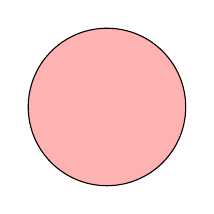
\begin{tikzpicture}
        \draw[fill=red!30] (0,0) circle (1);
    \end{tikzpicture}
    \caption{A circle}
    \label{fig:circle}
\end{subfigure}
\hfill
\begin{subfigure}[b]{0.3\textwidth}
    \centering
    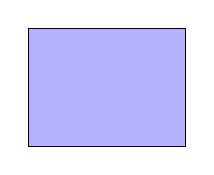
\begin{tikzpicture}
        \draw[fill=blue!30] (0,0) rectangle (2,1.5);
    \end{tikzpicture}
    \caption{A rectangle}
    \label{fig:rect}
\end{subfigure}
\hfill
\begin{subfigure}[b]{0.3\textwidth}
    \centering
    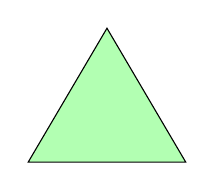
\begin{tikzpicture}
        \draw[fill=green!30] (0,0) -- (2,0) -- (1,1.7) -- cycle;
    \end{tikzpicture}
    \caption{A triangle}
    \label{fig:tri}
\end{subfigure}

\caption{Three shapes side by side. Refer to individual subfigures:
    (\subref{fig:circle}), (\subref{fig:rect}), (\subref{fig:tri}).}
\label{fig:shapes}
\end{figure}

See Figure~\ref{fig:shapes} for all three shapes, or
Figure~\ref{fig:circle} for just the circle.

% =============================================================================
\section{Float Placement Specifiers}
% =============================================================================

LaTeX float specifiers control where figures and tables appear:

\begin{center}
\begin{tabular}{cl}
    \textbf{Specifier} & \textbf{Meaning} \\
    \hline
    \texttt{h} & Place approximately \emph{here} \\
    \texttt{t} & Top of the page \\
    \texttt{b} & Bottom of the page \\
    \texttt{p} & On a separate float page \\
    \texttt{H} & Exactly here (requires \texttt{float} package) \\
    \texttt{!} & Override LaTeX's internal restrictions \\
\end{tabular}
\end{center}

Combine them: \verb|\begin{figure}[htbp]| tries here, then top, then bottom,
then a float page.

% =============================================================================
\section{Wrapping Text Around Figures}
% =============================================================================

The \texttt{wrapfig} package lets text flow around a figure:

\begin{wrapfigure}{r}{0.35\textwidth}
    \centering
    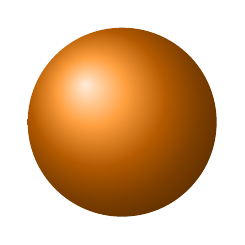
\begin{tikzpicture}
        \shade[ball color=orange] (0,0) circle (1.2);
    \end{tikzpicture}
    \caption{A wrapped figure.}
    \label{fig:wrapped}
\end{wrapfigure}

\lipsum[1]

% =============================================================================
\section{Forcing Float Position}
% =============================================================================

When you absolutely need a figure at a specific location, use \verb|[H]|
from the \texttt{float} package:

\begin{figure}[H]
\centering

\begin{tikzpicture}
    \draw[thick, fill=yellow!20] (0,0) -- (4,0) -- (4,2) -- (0,2) -- cycle;
    \node at (2,1) {\textbf{Exactly Here}};
\end{tikzpicture}
\caption{This figure is forced to appear exactly at this point.}
\label{fig:forced}
\end{figure}

\lipsum[2]

\end{document}
